\section{Results}
\label{sec:results}

Cyclic seam routing is held fixed; what varies is spherical
energy, always-on semantic energy, or the content-conditioned
gate.

\subsection{RQ1: How does ERP geometry affect seam routing?}
\label{sec:spherical}

Cyclic routing sets the legal neighbors
($\{x-1,x,x+1\}\bmod W$) as in~\eqref{eq:dp}, while spherical
energy~\eqref{eq:ep} rescales the cost of those neighbors. On
CVRG-Pano val+test ($n=120$), both sides use cyclic DP, $k=24$,
$W\le 512$, and $\lambda_s=0$, so only Sobel versus
$E_p=E_g\cos\phi$ changes. Polar occupancy is fixed by the
$15\%$ caps ($0.297$); the spherical signal is polar routing
share.

\begin{table}[t]
\centering
\caption{Polar routing on CVRG-Pano val+test ($n=120$, $k=24$).
Both rows use cyclic routing; only~\eqref{eq:ep} changes.
Values are mean${}\pm{}$std.}
\label{tab:spherical}
\small
\setlength{\tabcolsep}{3pt}
\resizebox{\columnwidth}{!}{%
\begin{tabular}{lccc}
\toprule
Method & Occupancy & Routing share & Mean polar $|\Delta x|$ \\
\midrule
Plain Sobel, cyclic & $0.297\pm 0$ & $0.301\pm 0.015$ & $0.766$ \\
Sobel $\times\cos\phi$, cyclic & $0.297\pm 0$ & $0.306\pm 0.014$ & $0.772$ \\
Paired $\Delta$ & $0.000$ & $+0.0042\pm 0.007$ & $+0.007$ \\
\bottomrule
\end{tabular}}
\end{table}

Occupancy is bit-identical, while routing rises from $0.301$ to
$0.306$ ($\Delta=+0.42$\,pp; $89/120$ up, $31$ down) and mean
polar step moves $+0.007$\,px. Only $23/120$ images move by more
than $+1$\,pp, and the unweighted polar/equator Sobel ratio is
uncorrelated with $\Delta$ (Spearman $\rho=-0.01$;
Fig.~\ref{fig:c1-scatter}). On this corpus the spherical term is
therefore a small routing shift.

\begin{figure}[t]
  \centering
  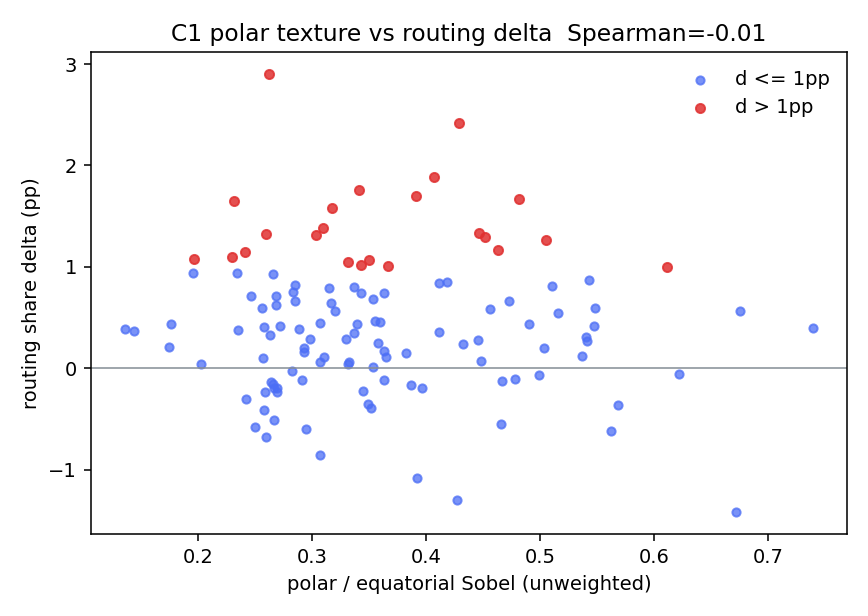
\includegraphics[width=0.82\linewidth]{figures/fig_c1_polar_scatter.png}
  \caption{Unweighted polar/equator Sobel ratio versus polar
  routing $\Delta$ on CVRG-Pano ($n=120$). Spearman
  $\rho=-0.01$. Red points: $\Delta>+1$\,pp.}
  \label{fig:c1-scatter}
\end{figure}

\subsection{RQ2: When does semantic protection matter?}
\label{sec:head-disks}

Always-on protection of $2^\circ$ GT head disks~\eqref{eq:rphi}
on PanoCount val+test, $k=24$, yields a limited aggregate
reduction (Table~\ref{tab:head-disks}): medium falls from
$4.3\%$ to $0.1\%$ ($\Delta=-4.18$\,pp), with (c)$<$(b) on
$82/171$ images. The pre-specified support bar was at least
$5$\,pp and a majority of images with (c)$<$(b); medium misses
both. Medium (b) already hits only $4.3\%$ of heads, so
$-4.18$\,pp uses essentially that range, while (c) improves on
(b) at $k=24$ on all $313$ images. $k=48$ would give $-8.73$\,pp
on medium. Scoring the same (b) seams against body columns
places medium at $12.6\%$. Fig.~\ref{fig:head-max}(a)--(b) shows
the largest medium head-hit reduction; $87/171$ medium frames are
$0\to 0$.

\begin{table}[!b]
\centering
\caption{Always-on $2^\circ$ GT head-disk protection, PanoCount
val+test, $k=24$. (b)/(c) are head-hit rates.}
\label{tab:head-disks}
\setlength{\tabcolsep}{3.5pt}
\small
\begin{tabular}{lrrrrrr}
\toprule
Bin & $N$ & (b) & (c) & $\Delta$ (pp) & (c)$<$(b) & Eq.\ cover \\
\midrule
Sparse $0$--$49$ & $72$ & $4.5\%$ & $0.1\%$ & $-4.39$ & $26/72$ & $0.8\%$ \\
Medium $50$--$199$ & $171$ & $4.3\%$ & $0.1\%$ & $-4.18$ & $82/171$ & $2.2\%$ \\
Dense $200+$ & $70$ & $3.7\%$ & $0.0\%$ & $-3.64$ & $31/70$ & $5.3\%$ \\
\bottomrule
\end{tabular}
\end{table}

\begin{figure*}[t]
  \centering
  \begin{minipage}[t]{0.495\linewidth}
    \centering
    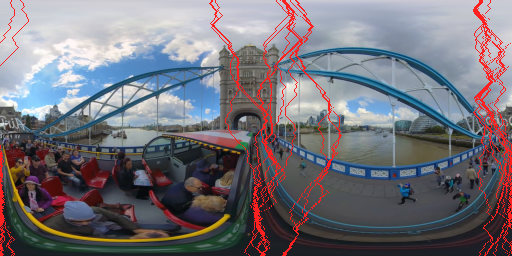
\includegraphics[height=3.15cm,keepaspectratio]{figures/fig_head_max_b.png}\\
    {\scriptsize (a) Head disks, spherical (b)}
  \end{minipage}\hfill
  \begin{minipage}[t]{0.495\linewidth}
    \centering
    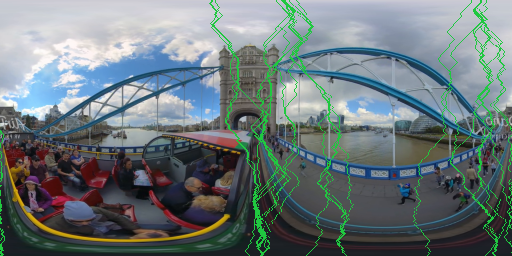
\includegraphics[height=3.15cm,keepaspectratio]{figures/fig_head_max_c.png}\\
    {\scriptsize (b) Head disks, $2^\circ$ energy (c)}
  \end{minipage}\\[3pt]
  \begin{minipage}[t]{0.495\linewidth}
    \centering
    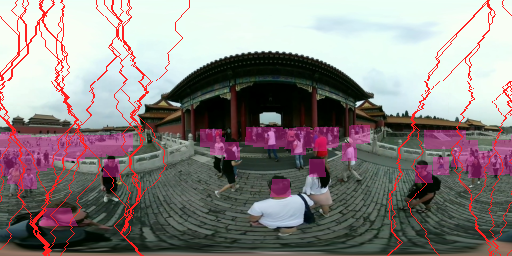
\includegraphics[height=3.15cm,keepaspectratio]{figures/fig_body_seams_b.png}\\
    {\scriptsize (c) Body columns, spherical (b)}
  \end{minipage}\hfill
  \begin{minipage}[t]{0.495\linewidth}
    \centering
    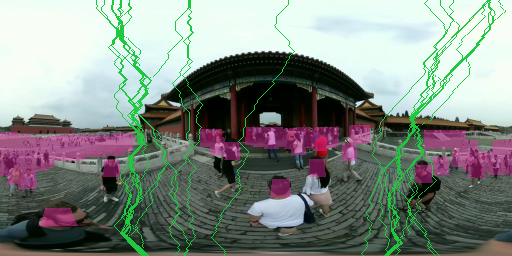
\includegraphics[height=3.15cm,keepaspectratio]{figures/fig_body_seams_c.png}\\
    {\scriptsize (d) Body columns, GT energy (c)}
  \end{minipage}
  \caption{Largest-change ERP examples at $k=24$. (a)--(b)~PanoCount
  medium, always-on $2^\circ$ GT head-disk energy. Red: spherical
  baseline. Green: (c). (c)--(d)~Largest oracle high-body case.
  Magenta: constructed GT body columns. Red: spherical baseline.
  Green: always-on $\lambda_s=4$.}
  \label{fig:head-max}
  \label{fig:body-seams}
\end{figure*}

\subsection{Content-Conditioned Semantic Protection}
\label{sec:body-boundary}

Body-column energy, $k=24$, paints GT heads as meridian strips
$12^\circ$ down, half-width $2.5\times$ the $2^\circ$ radius.
High-body is locked from (b) before (c) as the medium images
whose spherical seams already hit at least $20\%$ of those
columns ($n=49$), with complement $n=122$.
Table~\ref{tab:conditioned}(A) is an \emph{oracle}: energy and
split both see GT columns.

On oracle high-body, (c) drives GT body-hits from $35.4\%$ to
$0.2\%$ ($-35.2$\,pp) on every image. On the complement, (b)
already hits $3.4\%$, so (c) uses that ceiling ($-3.4$\,pp).
Fig.~\ref{fig:body-seams}(c)--(d) shows the largest oracle
high-body example.

\subsubsection{Practical gate}
The practical gate uses SegFormer-B0 ADE20K person instances
(Section~\ref{sec:setup}), $\tau=0.20$, and $k=24$
(Algorithm~\ref{alg:ccsc}). On PanoCount medium ($n=171$) it
turns $\lambda_s$ on for $56$ images and off for $115$
(Table~\ref{tab:conditioned}(A)), and mean GT body-hit falls from
$12.59\%$ to $11.04\%$ ($\Delta=-1.55$\,pp, $95\%$ CI
$[-2.75,-0.35]$). On the $56$ ON images the same metric changes
by $-4.73$\,pp (CI $[-8.28,-1.19]$): $34/56$ down, $5/56$ tied,
and $17/56$ up (Fig.~\ref{fig:qual}d). Gate-off $\Delta=0$ by
construction. The ON set overlaps oracle high-body on $30/49$
and misses $19/49$; it also fires on $26$ images outside that
subset. Always-on predicted-person instance hit falls from
$18.68\%$ to $5.16\%$ (Table~\ref{tab:conditioned}(B)). Extended
notes on the selection rule are in the supplementary material.

\subsection{Temporal Validation}
\label{sec:sparse-sampling}

Equatorial phase correlation~\cite{reddy1996fft} on one ERP2
frame ($I_t$, source $1626$, $W=512$) recovers a known cyclic
yaw exactly with zero post-warp residual, reports pan $0$ on the
next video frame ($\Delta t=0.03$\,s), and at a $7.74$\,s
linspace gap reports $253$\,px on the worst pair while the
residual ratio remains $0.95$. Sparse sampling can therefore
fabricate unsupported apparent yaw. Consecutive-frame windows of
ERP2, ERP4, and ERP5 in this corpus agree near zero;
Fig.~\ref{fig:c3-control} shows the three-condition control.

\begin{figure}[!b]
  \centering
  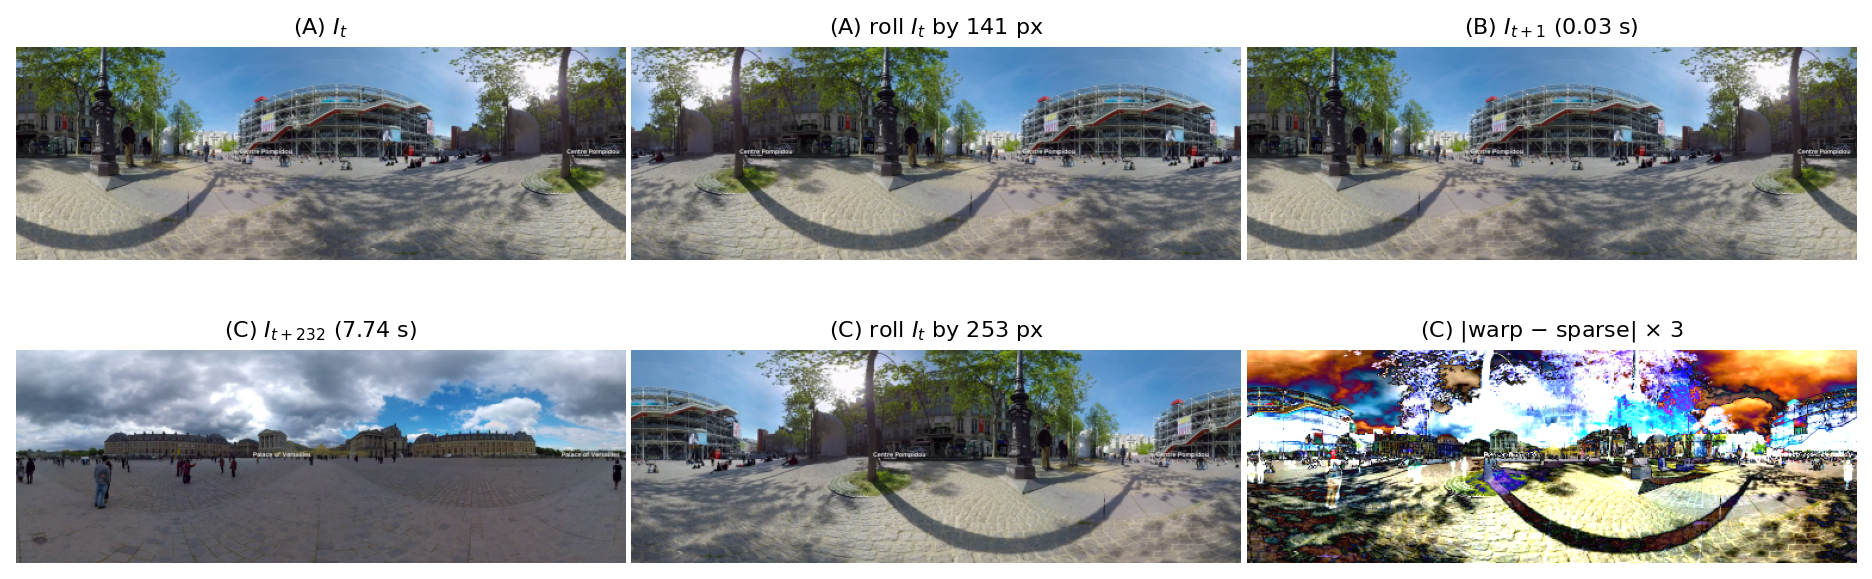
\includegraphics[width=\columnwidth]{figures/fig_c3_control.png}
  \caption{Same ERP frame $I_t$ (clip ERP2, source $1626$),
  equatorial band. (A)~A known $141$\,px cyclic roll is recovered
  exactly. (B)~The next video frame is already aligned (pan~$0$).
  (C)~At $7.74$\,s the estimator reports $253$\,px, but rolling
  $I_t$ by that amount leaves residual ratio $0.95$. Photometric
  residual is the validation criterion.}
  \label{fig:c3-control}
\end{figure}

\subsection{Qualitative Results}
\label{sec:qualitative}

Fig.~\ref{fig:qual} shows four medium PanoCount cases, with
magenta SegFormer predicted person pixels, red spherical (b)
seams, and green gated output. Stem $166$ is gate OFF with GT
$0$; stem $242$ is gate OFF with residual GT body-hit $16.9\%$;
stem $800$ is gate ON with GT down ($26.7\%\rightarrow 15.5\%$),
one of $34/56$; and stem $915$ is gate ON with GT up
($11.7\%\rightarrow 22.3\%$), one of $17/56$.

\begin{table*}[t]
\centering
\caption{Oracle versus practical content-conditioned protection
on PanoCount medium, $k=24$. (A)~GT body-hit (\% of constructed
GT persons). (B)~predicted-person instance hit (\% of SegFormer
components). $\Delta$ in percentage points. CI is~\eqref{eq:ci}.
A dash (---) marks rows where a CI was omitted. Panels are different
metrics.}
\label{tab:conditioned}
\label{tab:body-boundary}
\label{tab:practical-gate}
\setlength{\tabcolsep}{2.8pt}
\scriptsize
\begin{tabular}{l r r c c c c}
\toprule
\multicolumn{7}{l}{\textbf{(A)} Evaluation: GT body-hit} \\
\midrule
Method & $N$ & Gate ON & Before & After & $\Delta$ (pp) & $95\%$ CI \\
\midrule
Oracle high-body$^{\mathrm{a}}$ & $49$ & $49$ & $35.4\%$ & $0.2\%$ & $-35.2$ & --- \\
Oracle complement$^{\mathrm{a}}$ & $122$ & $0$ & $3.4\%$ & $0.0\%$ & $-3.4$ & --- \\
Practical predicted gate (all medium)$^{\mathrm{b}}$ & $171$ & $56$ & $12.59\%$ & $11.04\%$ & $-1.55$ & $[-2.75,-0.35]$ \\
Practical gate ON subset$^{\mathrm{b}}$ & $56$ & $56$ & $23.64\%$ & $18.90\%$ & $-4.73$ & $[-8.28,-1.19]$ \\
Practical gate OFF subset$^{\mathrm{b}}$ & $115$ & $0$ & $7.21\%$ & $7.21\%$ & $0$ & --- \\
\midrule
\multicolumn{7}{l}{\textbf{(B)} Evaluation: predicted-person instance-hit$^{\mathrm{b}}$} \\
\midrule
Always-on predicted-person$^{\mathrm{c}}$ & $171$ & $171$ & $18.68\%$ & $5.16\%$ & $-13.52$ & --- \\
\bottomrule
\end{tabular}

\vspace{4pt}
\begin{minipage}{\linewidth}
\raggedright\scriptsize
$^{\mathrm{a}}$GT-derived columns. Oracle After is always-on (c)
on the subset.\\
$^{\mathrm{b}}$SegFormer-B0 ADE20K person components. Practical
After is gated except in panel~(B).\\
$^{\mathrm{c}}$Always-on predicted-person instance hit.
\end{minipage}
\end{table*}

\begin{figure*}[t]
  \centering
  \begin{minipage}[t]{0.495\linewidth}
    \centering
    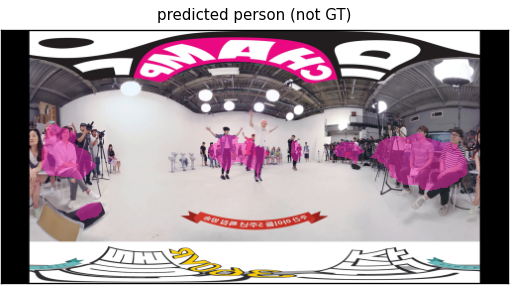
\includegraphics[width=0.325\linewidth]{figures/fig_qual_166_pred.png}%
    \hfill
    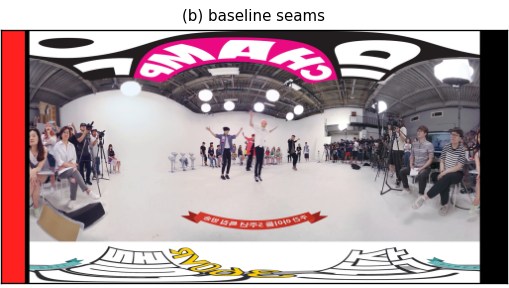
\includegraphics[width=0.325\linewidth]{figures/fig_qual_166_b.png}%
    \hfill
    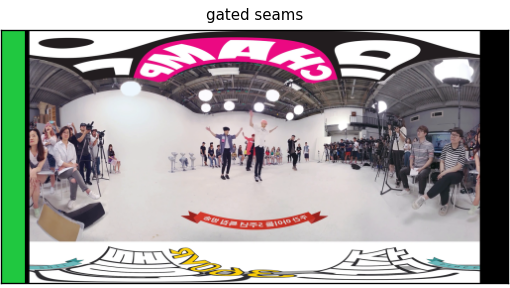
\includegraphics[width=0.325\linewidth]{figures/fig_qual_166_g.png}\\
    {\scriptsize (a) Stem $166$, OFF.
      $h_{\mathrm{pred}}=0$, GT $0\rightarrow 0$.}
  \end{minipage}\hfill
  \begin{minipage}[t]{0.495\linewidth}
    \centering
    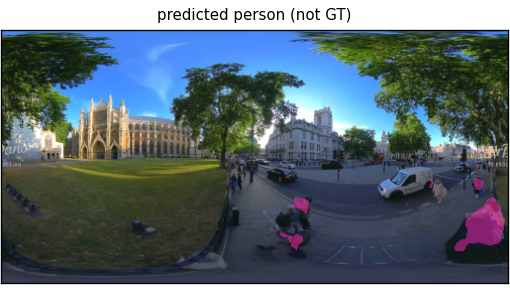
\includegraphics[width=0.325\linewidth]{figures/fig_qual_242_pred.png}%
    \hfill
    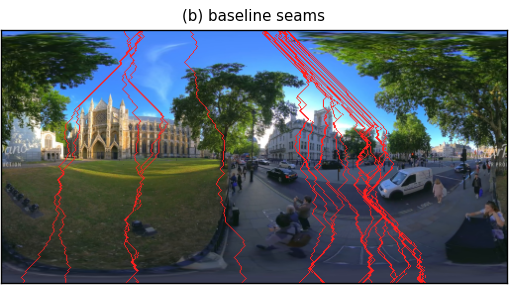
\includegraphics[width=0.325\linewidth]{figures/fig_qual_242_b.png}%
    \hfill
    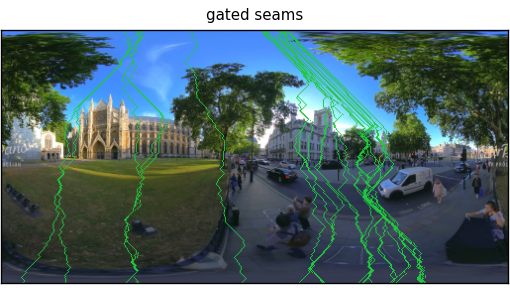
\includegraphics[width=0.325\linewidth]{figures/fig_qual_242_g.png}\\
    {\scriptsize (b) Stem $242$, OFF.
      $h_{\mathrm{pred}}=0$, GT remains $16.9\%$.}
  \end{minipage}\\[5pt]
  \begin{minipage}[t]{0.495\linewidth}
    \centering
    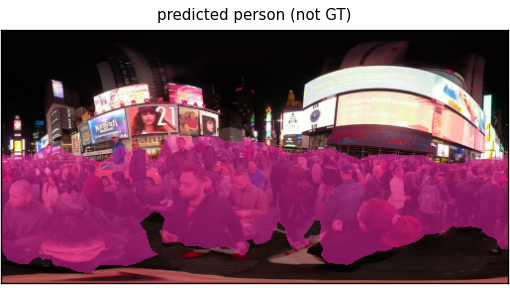
\includegraphics[width=0.325\linewidth]{figures/fig_qual_800_pred.png}%
    \hfill
    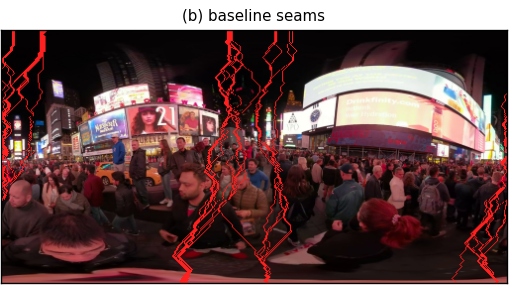
\includegraphics[width=0.325\linewidth]{figures/fig_qual_800_b.png}%
    \hfill
    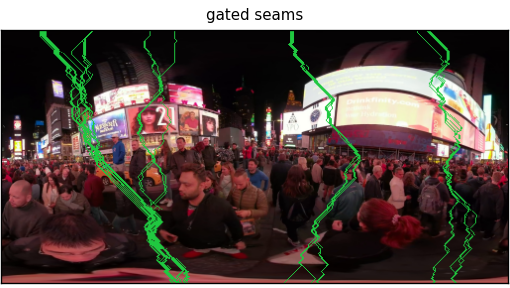
\includegraphics[width=0.325\linewidth]{figures/fig_qual_800_g.png}\\
    {\scriptsize (c) Stem $800$, ON.
      GT $26.7\%\rightarrow 15.5\%$.}
  \end{minipage}\hfill
  \begin{minipage}[t]{0.495\linewidth}
    \centering
    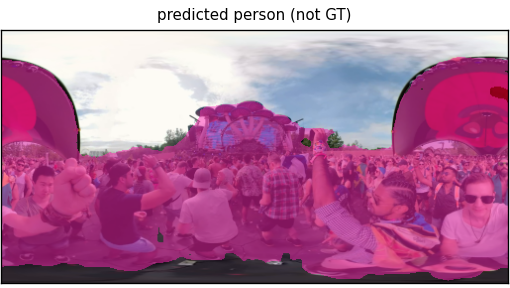
\includegraphics[width=0.325\linewidth]{figures/fig_qual_915_pred.png}%
    \hfill
    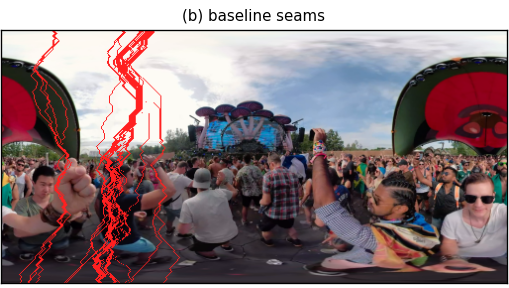
\includegraphics[width=0.325\linewidth]{figures/fig_qual_915_b.png}%
    \hfill
    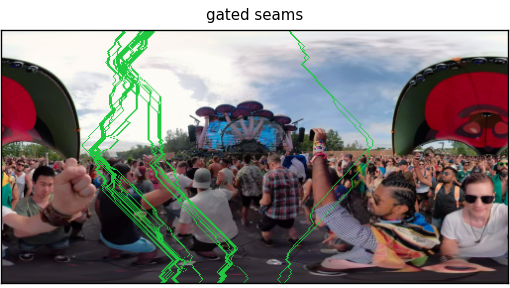
\includegraphics[width=0.325\linewidth]{figures/fig_qual_915_g.png}\\
    {\scriptsize (d) Stem $915$, ON.
      GT $11.7\%\rightarrow 22.3\%$.}
  \end{minipage}
  \caption{Practical-gate cases on PanoCount medium. In each
  triplet, left is the predicted-person overlay, middle is
  spherical (b) seams, right is gated seams. Magenta:
  SegFormer-B0 ADE20K person pixels. Red: (b). Green: gated
  output. GT body-hit is the evaluation score;
  $h_{\mathrm{pred}}$ is the gate statistic.}
  \label{fig:qual}
\end{figure*}
